\documentclass[]{article}
\usepackage[spanish]{babel}
\usepackage{graphicx}
\usepackage[utf8]{inputenc}
\usepackage{fancyhdr}
\usepackage{lastpage}

\pagestyle{fancy}
\fancyhf{}
\rfoot{Page \thepage\hspace{1pt} de~\pageref{LastPage}}

\title{Practica 12}
\author{Guillermo Lopez Garcia}
\begin{document}
\maketitle

\textbf{Ejercicio 4.} \\

Como se puede apreciar en las imagenes siguientes, se muestran las comparativas de tiempo entre C++ y Java, tanto en windows
como en linux. A la conclusión a la que se llega, es que apenas existe diferencia apreciable. Parece ser, que windows ha
empezado a hacer bien las cosas.

\begin{figure}
  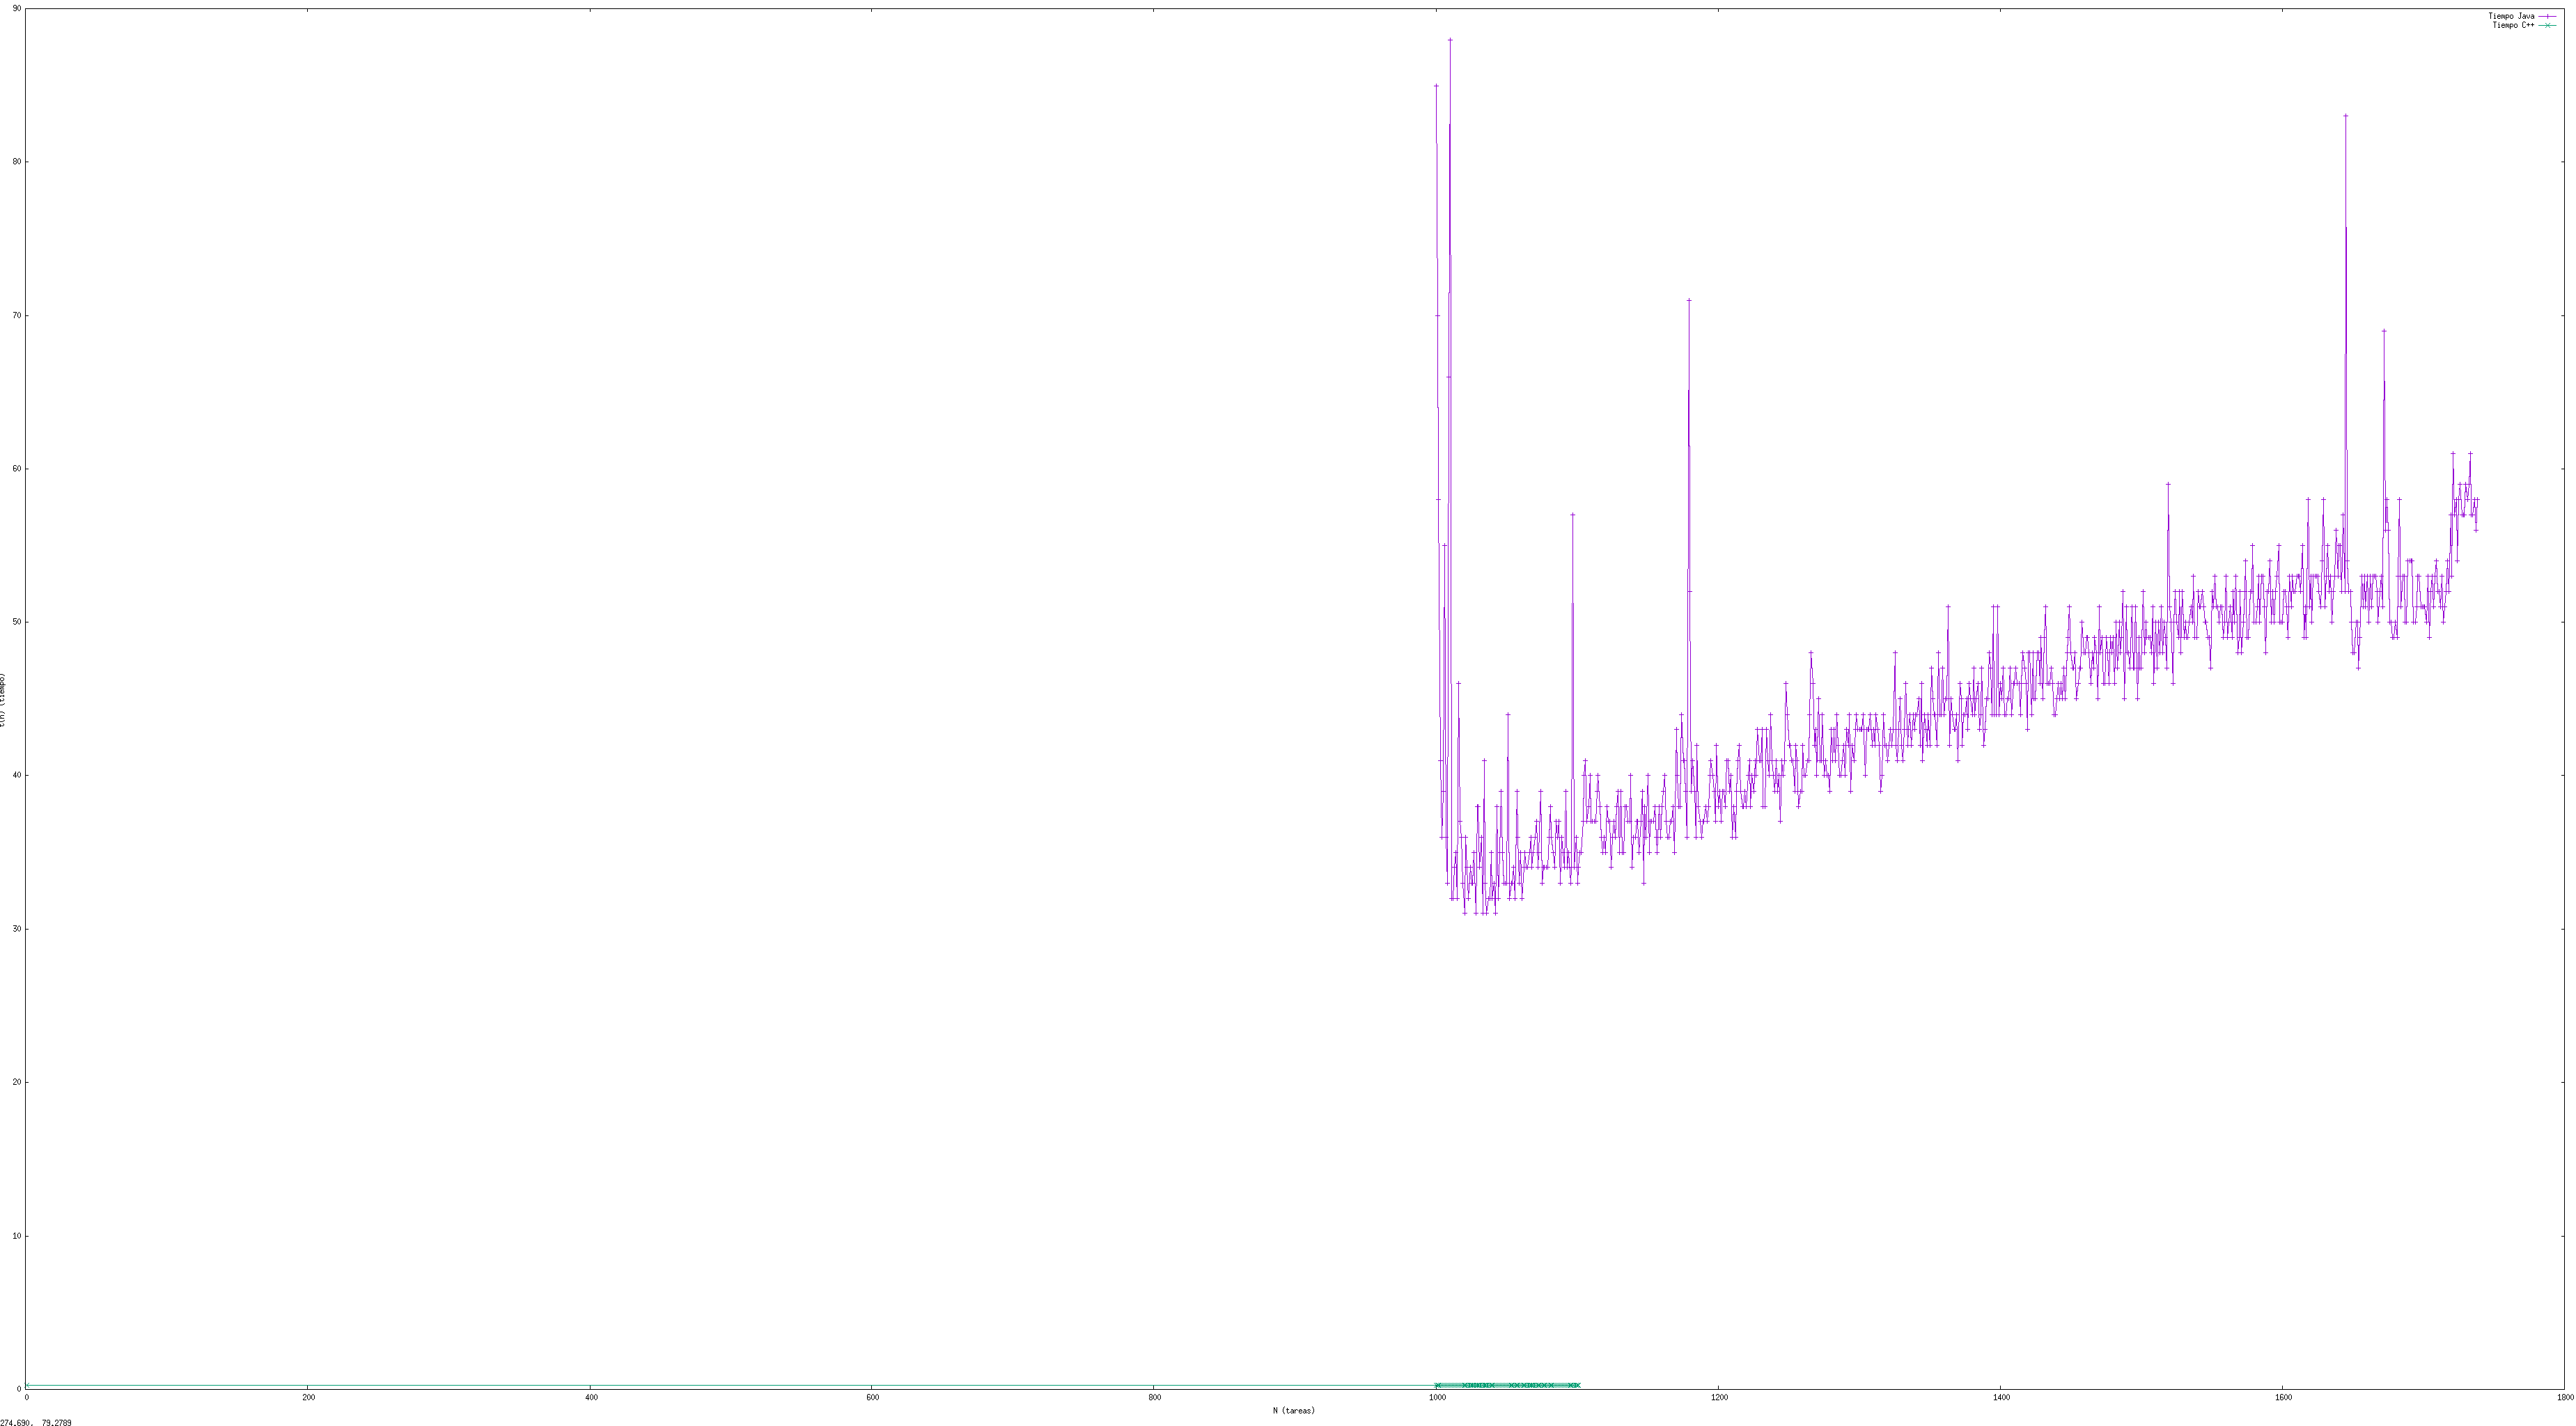
\includegraphics[width=\linewidth]{linux.png}
  \caption{Comparativa C++ y Java en Linux}
\label{fig:comp}
\end{figure}

\begin{figure}
  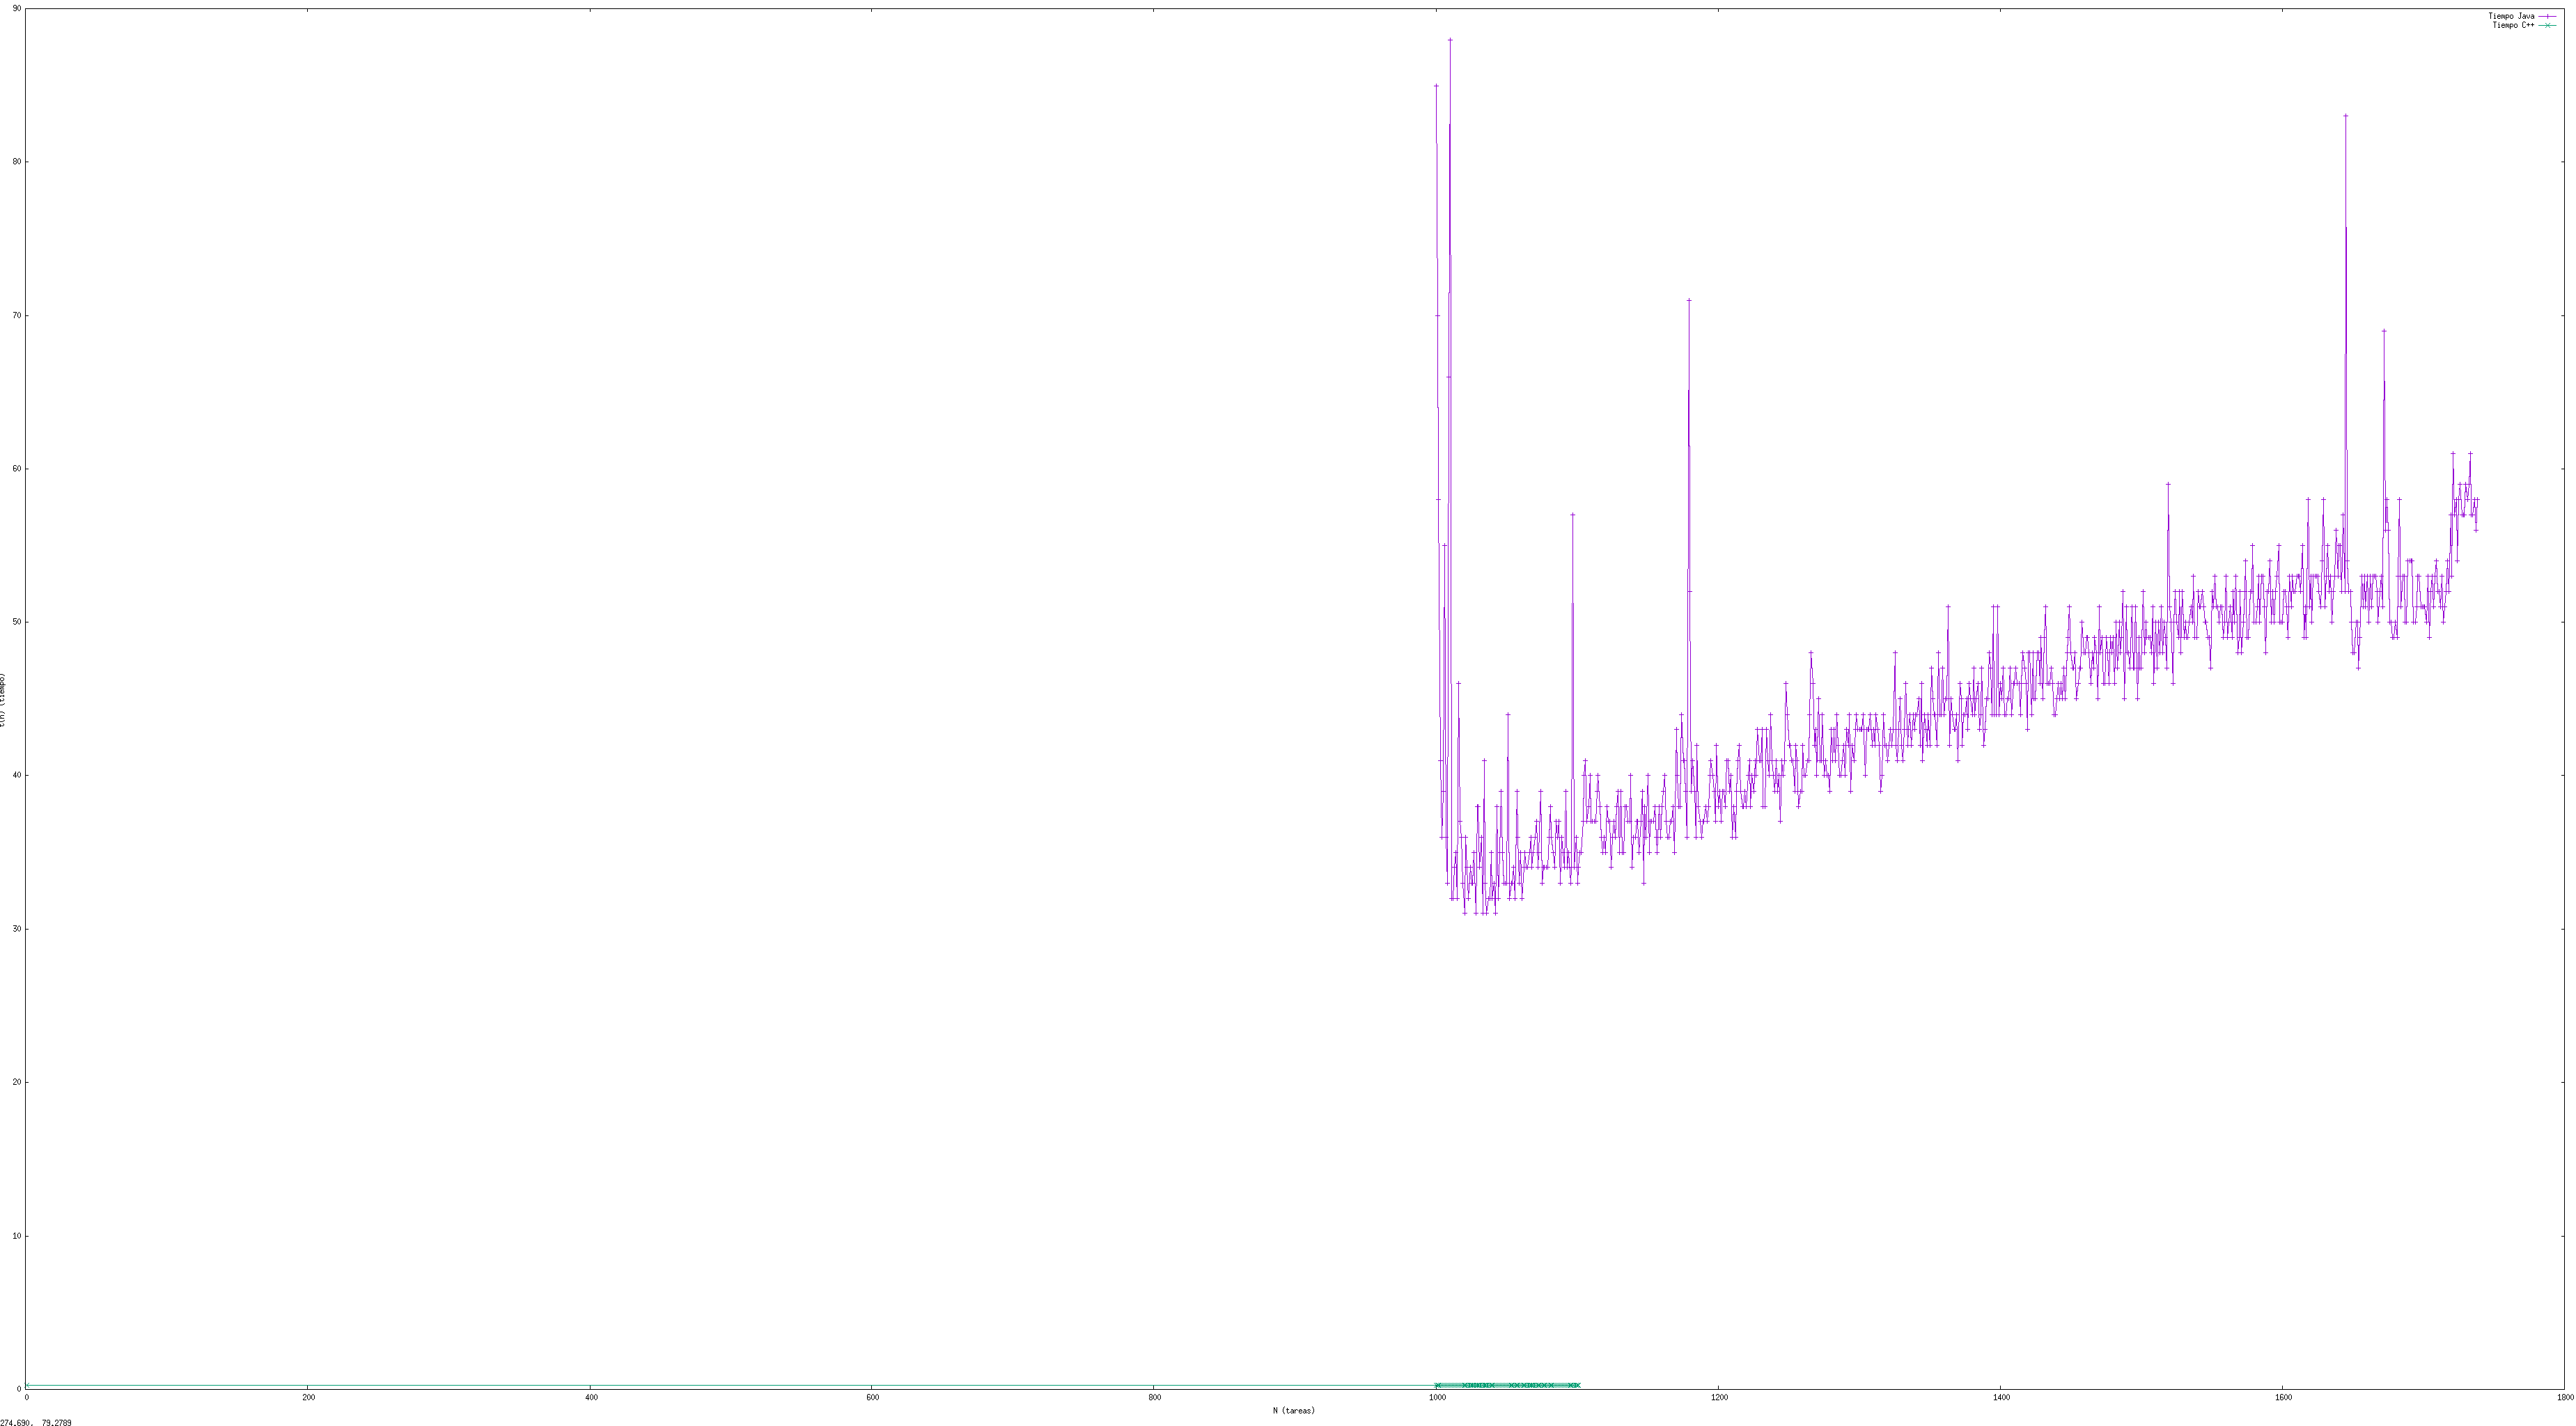
\includegraphics[width=\linewidth]{windows.png}
  \caption{Comparativa C++ y Java en Windows}
\label{fig:comp}
\end{figure}

\end{document}
